\documentclass[twoside,twocolumn,11pt]{article} %If no option is specified, 10pt is assumed

\usepackage[sc]{mathpazo} % Use the Palatino font
\usepackage[T1]{fontenc} % Use 8-bit encoding that has 256 glyphs
\linespread{1.05} % Line spacing - Palatino needs more space between lines
\usepackage{microtype} % Slightly tweak font spacing for aesthetics
\usepackage{csquotes}
\usepackage[english]{babel} % Language hyphenation and typographical rules
\usepackage{graphicx}
\usepackage{float}
\usepackage{wrapfig}
\usepackage{amsmath,amssymb}
\usepackage[hmarginratio=1:1,top=32mm,columnsep=20pt,margin=0.6in]{geometry} % Document margins, margin=0.6in wasn't there first.
\usepackage[hang, small,labelfont=bf,up,textfont=it,up]{caption} % Custom captions under/above floats in tables or figures
\usepackage{booktabs} % Horizontal rules in tables

\usepackage{lettrine} % The lettrine is the first enlarged letter at the beginning of the text

\usepackage{enumitem} % Customized lists
\setlist[itemize]{noitemsep} % Make itemize lists more compact

\usepackage{abstract} % Allows abstract customization
\renewcommand{\abstractnamefont}{\normalfont\bfseries} % Set the "Abstract" text to bold
\renewcommand{\abstracttextfont}{\normalfont\small\itshape} % Set the abstract itself to small italic text

\usepackage{titlesec} % Allows customization of titles
\renewcommand\thesection{\Roman{section}} % Roman numerals for the sections
\renewcommand\thesubsection{\roman{subsection}} % roman numerals for subsections
\titleformat{\section}[block]{\large\scshape\centering}{\thesection.}{1em}{} % Change the look of the section titles
\titleformat{\subsection}[block]{\large}{\thesubsection.}{1em}{} % Change the look of the section titles

\usepackage{fancyhdr} % Headers and footers
\pagestyle{fancy} % All pages have headers and footers
\fancyhead{} % Blank out the default header
\fancyfoot{} % Blank out the default footer
\fancyhead[C]{Electrical Steel: An investigation into the
brittleness of the Fe-Si alloy} % Custom header text
\fancyfoot[RO,LE]{\thepage} % Custom footer text

\usepackage{titling} % Customizing the title section
\usepackage{cite}
\usepackage{hyperref} % For hyperlinks in the PDF

\setlength{\headheight}{13.59999pt} % make fancyheader stop complaining
%----------------------------------------------------------------------------------------
%	TITLE SECTION
%----------------------------------------------------------------------------------------

\setlength{\droptitle}{-4\baselineskip} % Move the title up

\pretitle{\begin{center}\Huge\bfseries} % Article title formatting
\posttitle{\end{center}} % Article title closing
\title{Electrical Steel: An investigation into the
brittleness of the Fe-Si alloy} % Article title
\author{%
\textsc{Arthur Adriaens} \\[1ex] % Your name
\normalsize Ghent University \\ % Your institution
\normalsize \href{mailto:arthur.adriaens@ugent.be}{arthur.adriaens@ugent.be} % Your email address
\and % Uncomment if 2 authors are required, duplicate these 4 lines if more
\textsc{Cedric Ooms} \\[1ex] % Second author's name
\normalsize University of Antwerp \\ % Second author's institution
\normalsize \href{mailto:cedric.ooms@student.uantwerpen.be}{cedric.ooms@student.uantwerpen.be} % Second author's email address
\and % Uncomment if 2 authors are required, duplicate these 4 lines if more
\textsc{Chris Corentin} \\[1ex] % Second author's name
\normalsize Free University of Brussels \\ % Second author's institution
\normalsize \href{mailto:corentin.chris.m.mergny@vub.be}{corentin.chris.m.mergny@vub.be} % Second author's email address
}

\date{\today} % Leave empty to omit a date
\renewcommand{\maketitlehookd}{%
\begin{abstract}
\noindent 
In this paper, we'll hunt for ordered crystal structures that may be
stable, and that would explain the brittleness of electrical steel. We'll do
this by exploiting the advantage that ab initio simulations (done using Quantum
ESPRESSO (opEn-Source Package for Research in Electronic Structure,
Simulation, and Optimization) \cite{Giannozzi_2017} \cite{Giannozzi_2009} \cite{exoscaleqe}) give full control over defining
the crystal: We'll tell exactly where we want to have every atom, and quantum
chemistry will tell us what is the internal energy that corresponds to such
crystal. By modifying the positions of the atoms, and by monitoring the
corresponding internal energy, we may find ordered crystals that areo
thermodynamically stable. (This is, of course, only a draft)
\end{abstract}
}

%----------------------------------------------------------------------------------------

\begin{document}

% Print the title
\maketitle

%----------------------------------------------------------------------------------------
%	ARTICLE CONTENTS
%----------------------------------------------------------------------------------------

\section{Introduction}
%The sec:level1 means first level section, as opposed to second, third,...
% Third level is achieved via the usual subsubsection
Electric applications such as motors, transformers or generators all have a magnetic material in the core of their electromagnetic coil. Almost always, this is a so-called electrical steel: a Fe-Si alloy with about 3 wt.\% Si.
It is known since
decades that using a steel with 6.5 wt.\% Si would be very advantageous[citation needed] over the steel we're now using. Such a steel would
reduce energy losses in the application, which would make it possible to build electric machines lighter and more
energy efficient. Estimates come up with a saving of several billions of euro worth of electricity every
year [citation needed].
So why aren't we using that ideal electrical steel? In contrast to 3 wt.\% Si, the 6.5 wt.\% Si steel is
brittle: you can’t press or roll or otherwise form it into the size and shape needed to build the electric
apparatus. It would just break apart when trying to do so. Hence finding an electrical steel with 6.5 wt.\% Si
that is not brittle is quite the holy grail in electrical steel research.
There is a hypothesis about why the brittleness appears. Crystals with long range order are usually
more brittle than crystals in which the atoms are more disordered [citation needed]. It is assumed that when
increasing the silicon content, there is a stronger tendency for the atoms to develop short-range
order.


\section{Convergence testing}
We'll be using the SPSS pseudopotentials\cite{doi:11.1126/science.aad3000} \cite{Prandini2018} for all of our calculations.
\subsection{bcc-Fe}
\begin{wrapfigure}{R}{0.1\textwidth}
  \begin{center}
	  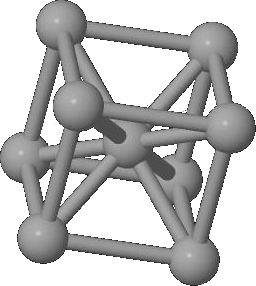
\includegraphics[width=0.1\textwidth]{figures/bcc-iron.png}
  \end{center}
\end{wrapfigure}
For bcc-Fe iron we use Patrick M. Woodward et.al's cif file. We're also using a pseudopotential generated using "atomic" code by A.
Dal Corso  v.5.0.99 svn rev. 10869 with the minimum cutoff for wavefunctions
being the suggested 64. Ry and the minimum cutoff for charge density the
suggested 782. Ry. We use the hydrostatic pressure to test the convergence, for different k-meshes we find the following:
\begin{table}[ht]
\begin{tabular}{c|c|c}
	& k mesh & Hydrostatic Pressure (kbar)\\
	\hline
	1&(1,1,1)&291.45\\
	2&(3,3,3)&76.49\\
	3&(5,5,5)&-99.45\\
	4&(7,7,7)&-71.98\\
	5&(9,9,9)&-109.31\\
	6&(10,10,10)&-98.83\\
	7&(11,11,11)&-80.23\\
	8&(13,13,13)&-92.67\\
	9&(15,15,15)&-84.76\\
\end{tabular}
\end{table}\\
We find it has sufficiently converged at (10,10,10) so that's the k-mesh we'll
be using. Now keeping the cutoff charge density $\approx 12$ times the cutoff
for wavefunctions, we'll vary this wavefunction cutoff: \begin{table}[ht]
\begin{tabular}{c|c|c}
	&ecutwfc&Hydrostatic Pressure (kbar)\\
	\hline
	1&14&-15244\\
	2&24&-1727\\
	3&34&-962\\
	4&44&-457\\
	5&54&-95\\
	6&64&-98\\
\end{tabular}
\end{table}\\
Here we see quite a good convergence at ecutwfc = 54, we'll now take ecutwfc=54 and vary the multiplicity of the charge density:
\begin{table}[ht]
\begin{tabular}{c|c|c|c}
	&factor&ecutrho&Hydrostatic Pressure (kbar)\\
	\hline
	1&2&108&939\\
	2&4&216&0.81\\
	3&6&324&-69\\
	4&8&432&-96\\
	5&10&540&-92\\
	6&12&648&-95\\
\end{tabular}
\end{table}\\
We already see convergence at a factor 8. Our final values are thus a k-mesh of (10,10,10), ecutwf at 54 and ecutrho at 432.
\subsection{DO3-Fe3Si}
\begin{wrapfigure}{L}{0.1\textwidth}
  \begin{center}
	  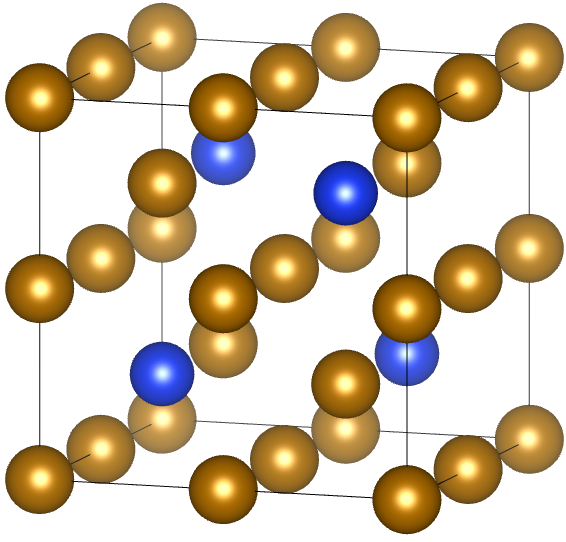
\includegraphics[width=0.1\textwidth]{figures/DO3-Fe3Si_transl_no_background.png}
  \end{center}
\end{wrapfigure}
DO3-Fe$_3$Si is the name of the crystal with a unit cell built from 8 bcc-Fe
unit cells stacked in a 2x2x2 way, to make a cube with twice the edge length of
a normal bcc-Fe unit cell. Herein every other unit cell's middle iron nucleus
is replaced with a Si nucleus, such that these 4 atoms form a tetrahedron. This
is a bit hard to recognize in the figure on the left\footnote{cif file by Farquhar M. C. M.,
Lipson H. and Weill A. R., with COD index 9015110} as that one is shifted up
and to the left, but this is in fact the same compound.
We thus have a unit cell with 16 atoms of which 4 are Si atoms, giving us a concentration of 25 at.\% $\approx$ 14.36 wt.\%.
Let's now do the same procedure as with bcc-Fe, we wish to have a k-mesh,
ecutwf and ecutrho that will work for both so we can later on ignore these
parameters. The unit cell has doubled in size so the k-mesh should be halved
let's see if we thus get convergence at (5,5,5). Starting with ecutwfc=64 and
ecutrho=782 as these, the minimal values for the Fe pseudopotential, are higher
than the ones in the Si pseudopotential:
\begin{table}[ht]
\begin{tabular}{c|c|c}
	&k mesh&Hydrostatic Pressure (kbar)\\
	\hline
	1&(3,3,3)&-88\\
	2&(4,4,4)&-43\\
	3&(5,5,5)&-71\\
	4&(6,6,6)&-63\\
	5&(7,7,7)&-73\\
\end{tabular}
\end{table}\\
We "again" see convergence at (5,5,5). Now again keeping the cutoff charge density 12 times the cutoff
for the amount of wavefunctions and varying the charge density:
\begin{table}[ht]
\begin{tabular}{c|c|c}
	&ecutwfc&Hydrostatic Pressure (kbar)\\
	\hline
	1&14&-11640\\
	2&24&-1350\\
	3&34&-770\\
	4&44&-355\\
	5&54&-68\\
	6&64&-71\\
\end{tabular}
\end{table}\\
I.e we again see convergence at ecutwfc=54. Let's now search the multiplication factor:
\begin{table}[ht]
\begin{tabular}{c|c|c}
	&ecutwfc&Hydrostatic Pressure (kbar)\\
	\hline
	1&14&-11640\\
	2&24&-1350\\
	3&34&-770\\
	4&44&-355\\
	5&54&-68\\
	6&64&-71\\
\end{tabular}
\end{table}\\
\begin{table}[ht]
\begin{tabular}{c|c|c}
	&factor&hydropressure\\
	\hline
	1&4&-12\\
	2&5&-61\\
	3&6&-50\\
	4&7&-63\\
	5&8&-68\\
\end{tabular}
\end{table}\\
We thus see convergence already at a factor of 5, so we'll take the highest factor of both, i.e 8. Our final 
values are thus ecutwfc=54, ecutrho at 432 and a k-mesh of (5,5,5).
\section{Energies of the end points}
We'll do a full geometry optimization by first using the
calculation="vc-relax" control parameter and bfgs cell and ion
dynamics with 0 pressure (0.5 kBar convergence threshold) for
both crystals.\\
We also did a manual optimization, as to also obtain an equation of state, from which a value for the bulk modulus is derived. To do this, static calculations at 5 slightly different lattice parameters were done, after which a vc-relax calculation with target pressure equal to the weighted average of each of the previously obtained stress tensors was performed. This data was used then used to fit a Birch-Murnaghan equation of state.

\subsection{bcc-Fe}
Using the first method, for bcc-Fe we get a final total energy of
-329.26 Ry for a unit cell containing 1 atom with a unit cell volume
of 76.1642 a.u.$^3$ $\implies$ cell length of 4.238871 au, or a
length of 0.492942382 alat with a 2.999754 scale.\\ Using the second
method a unit cell volume of 76.52 a.u.$^3$, was found, with lattice
parameter 5.35 a.u. = 2.84 \AA. This corresponds again with an
energy of -329.26 Ry. Using the Birch-Murnaghan fit a value for the
bulk modulus of 176.0 GPa was obtained (value on
materialsproject.org is 182 GPa).
\subsection{DO3-Fe3Si}
For Fe$_3$Si we get a final total energy of -999.30084673 Ry for a
unit cell containing 4 atoms with a volume of 296.49363 a.u.$^3$

Using the second method a unit cell volume of 301.56 a.u.$^3$ was found. This corresponds with an energy of -999.30170 Ry. Using the Birch-Murnaghan fit a value of 190.3 GPa was found for the bulk modulus (value on materialsproject.org is 212 GPa).

\section{Sanity Check}
We'll take the DO3-Fe$_3$Si and change 1 Silicon atom in the unit
cell to an Fe atom, for this we'll first have to remove the 
symmetry and define all the atom's coordinates ourselves.
The DO3-Fe$_3$Si crystal has F m -3 m as symmetry space group
(number 225). Looking at the crystallographic database
we see that the first Fe atom to consider which has relative atomic 
position (0.5 0.5 0.5) corresponding to Wyckoff Position 4b,
the second one has Wyckoff Position 8c and the Si atom has 4a.
I.e our unit cell has 4+8+4 = 16 atoms which is correct.
\newline
Making a cif file without symmetry can then be done quite
straightforwardly. We then check if the energy we get is indeed the
same. The energy we get from our Fe$_3$Si crystal without symmetry
is -3997.2 Ry per 16 atom unit cell or -999.3 Ry per 4 which is the
same as we found earlier, this is thus a good input file to modify,
we'll now replace one Si atom with Iron as shown in figure
\ref{fig:Sanity}.
\begin{figure}
	\centering
	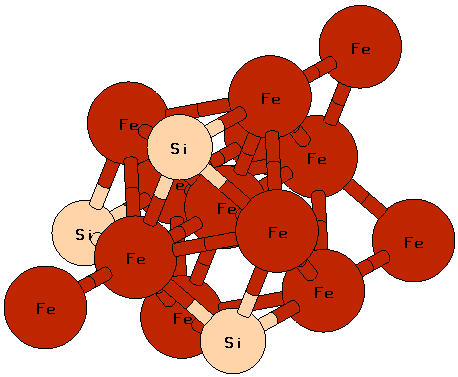
\includegraphics[width=0.3\textwidth]{figures/Sanitynolight.png}
	\caption{DO3-Fe$_3$Si with 1 Silicon changed to Iron}
	\label{fig:Sanity}
\end{figure}
Doing this gives us a 18.75 at.\% $\equiv$ 10.40 wt.\% Si crystal.
After a 'vc-relax' calculation we get an energy of about -4314.944
Ry, this crystal can be composed of 3 Fe$_3$Si (containing 4 atoms)
and 4 Fe (containing 1 atom) unit cells giving a sum of energies of:
\begin{equation}
	3 \text{Fe}_3\text{Si} + 4 \text{Fe} = -( 3* 999.3 + 4*329.26) = 4314.94
\end{equation}
So almost exactly the same energy found by doing the simulation.
It won't decompose as it's energy is just a little lower than 
the weighted sum of the two.
%----------------------------------------------------------------------------------------
%	REFERENCE LIST
%----------------------------------------------------------------------------------------
\bibliography{sources}
\bibliographystyle{plain}

%----------------------------------------------------------------------------------------

\end{document}

